\documentclass{article}

\usepackage[T1]{fontenc}
\usepackage{graphicx}
\usepackage[a4paper, margin=2cm]{geometry}
\usepackage{hyperref}
\usepackage{lastpage}
\usepackage{fancyhdr}
\usepackage{datetime}
\usepackage{glossaries}

\hypersetup{
  colorlinks = true,
  urlcolor = blue,
  citecolor = black,
  linkcolor = black
}


\makeglossaries

\newglossaryentry{gmp}
{
  name=GMP,
  description={Good manufacturing practice}
}

\newglossaryentry{fdg}{name={FDG},description={[$^{18}$F]Fluorodeoxyglucose, a common radioactive tracer used for PET images}}

\newglossaryentry{CIMT}{name={CIMT},description={Center for IT and Medico technologies. Responsible department for IT in the Capital Region of Denmark}}

\newglossaryentry{git}{name={Git},description={Git is a free and open source distributed version control system designed to handle everything from small to very large projects with speed and efficiency. Found at \url{https://git-scm.com}}}
\newglossaryentry{invalid state}{name={invalid state},description={This is a database}}

\newglossaryentry{invalid data}{name={invalid data},description={Nonsensical data that could never be valid. Examples include a reference to an nonexistent object or Negative halflife or activity}}
\newglossaryentry{incorrect data}{name={incorrect data},description={Data that doesn't reflect reality. Examples include a misspelled batch number or an activity entry which does not match actual activity in the vial}}

\graphicspath{{./figures/}}

\fancyhf{}
\fancyfoot[L]{\today}
\fancyfoot[R]{Page \thepage \, of \pageref{LastPage}}
\fancyhead[L]{Technical documentation \& Risk assessment of Tracershop}
\fancyhead[R]{Doc nr: <I'm a document Number>}
\pagestyle{fancy}

\author{Christoffer Vilstrup Jensen}
\title{Technical documentation}
\begin{document}


\begin{titlepage}
  \begin{minipage}{0.48\linewidth}
    
\includegraphics[width=0.6\linewidth]{logo.png}
  \end{minipage}
  \begin{minipage}{0.48\linewidth}
    \raggedleft
      
\includegraphics[width=0.6\linewidth]{petlogo_small.png}
  \end{minipage}
  \vspace{1cm}
  \begin{center}
    \Huge Technical documentation and risk assessment for Tracershop \\
    \vspace{1cm}
    \Large Christoffer Vilstrup Jensen\\
    MSc. Computer Science\\
  \end{center}
\end{titlepage}

\section*{Introduction}
This document describes the electronic bookkeeping system, Tracershop, used for ordering
and release of radioactive tracers for clinical procedures produced at Rigshospitalet's cyclotron unit.
Rigshospitalet delivers radioactive tracers to hospitals and scientific institutions near Copenhagen,
that would not be able to perform various PET scans without the tracers.
Therefore Tracershop should be considered a important piece of software.\\
The original tracershop was released in 2004 and in the field of Computer Science such a system is considered ancient.
This document contains an exploration of various risks with the old system and presents a replacement system with the aims to improve the user experience,
functionality, and improve IT-security, namely a react-django new web server and makes a risk assessment of the current and the new system.

\subsection*{Abstractions}
Tracershop handles two different types of orders. Activity based orders and Injection based orders.\\
An \textbf{activity order} is defined as an order, where a customer orders an amount of MBq radioactive tracer at a predetermined time slot known as a "deliver time".
It's the user responsibility to account for radioactive decay between injection time and delivery time.\\
An \textbf{injection order} is an order with a number of injections with a predefined amount of activity, and it's Tracershops responsibility to account for any decay between production time and injection time.
Users er limited per user basis which injection tracers they can order.

\subsection*{Requirements}

\begin{itemize}
  \item A user can order radioactive tracer from the internet while not connected to the Capital Region intranet.
  A user can be limited in their selection of tracers and limited time window where such tracers are available for ordering.
  \item A user can review any order they have made, and view batch number of tracer that they have ordered. They cannot view or alter order, which doesn't belong to them. They cannot alter delivered orders.
  \item A released order has a batch number and a record of who released it.
  \item Non authenticated users cannot alter or view information in tracershop.
\end{itemize}



\section*{Tracershop - Current system}
Since 2004, the software ecosystem is centered around a MySQL 5.1 database running on a openSUSE 11.2 distribution, which contains all the records and logs about the production of tracers. 
This database is back up on an external machine every day at midnight.\\
The web site is a Zope 2-2.13 web interface at \url{http://pet.rh.dk} allowing the users to systematically write to the main database.
It is normal that software is deprecated after a period of support, and keeping a software product up to date is part of the maintenance of a software products life cycle,
however that have not been possible due to insufficient resources.\\
An overview of the current system can be seen in figure \ref{fig:oldsys}.
\begin{figure}[ht]
  \begin{center}
    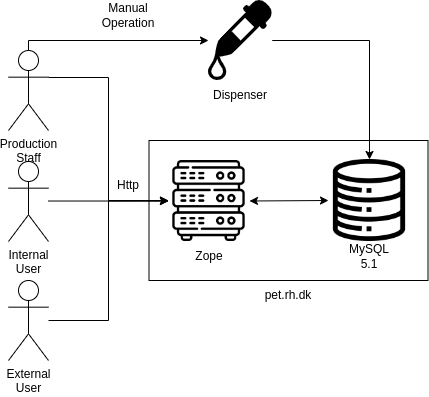
\includegraphics[width=0.6\linewidth]{OldSetup.png}
    \caption{Current Tracershop system}
    \label{fig:oldsys}
  \end{center}
\end{figure}


The dispenser ensures the amount of product in vials and the digital record of the product are equal.
The dispenser writes these records to it own database, which does not support multiple concurrent connections, making it impossible to retrieve them the conventional way.
A script circumvents this obstacle by opening the database as a file, and by using a byte offset retrieves the data of the dispensed vial.
This solution is highly fragile, and an update to the database could change the file format of the database.
This would render the script inoperable as the byte offset would no longer be correct.\\
Should the offset be incorrect the script would read garbage, so it could not construct a valid entry and thus would mostly likely fail.
In that event the production staff would have to manually read the data from the dispenser and then write the data into Tracershops database, which introduces another human error.\\
It's therefore recommended to replace the dispenser, with one fulfils the requirements of either:
\begin{itemize}
  \item Writes dispensed tracer data to a database that allows multiple connections.
  \item Writes dispensed tracer data to a file.
\end{itemize}
Currently it's the The Department of clinical physiology nuclear medicine which hosts the server.
Which is not desired because hosting server is a core task \GLS{CIMT} and not the clinical departments.


\subsection*{Database layout}
The Tables in the Tracershop main database, note the tables casing does not conform to the snake casing that standard for SQL databases:
\begin{enumerate}
  \item Log - Likely Zope related. No longer in use as the last entry was in 2010-03-18.
  \item MiscData - Likely Zope related. Likely a temporary value container.
  \item Roles - Zope related, defines different user roles in the Tracershop program.
  \item Sessions - Likely Zope related, defines active user sessions.
  \item Tokens - Likely Zope related, Likely defines the length of active sessions.
  \item TracerCustomer - Defines which user have access to order which injection Tracer.
  \item Tracers - Catalog of tracer available in tracershop.
  \item UserRoles - Relates user to a Role from the Role table.
  \item Users - All users able to be authenticated in tracershop
  \item VAL - Record of a vial with tracer, produced by the dispenser.
  \item VAL2 - Not in use.
  \item blockDeliverDate - Extraordinary dates where tracershop is closed, such a holydays.
  \item deliverTimes - Weekly points in time specifying when a customer can place an activity order.
  \item isotopes - Catalog of radioactive isotope used in the tracers.
  \item orders - List of activity orders.
  \item productionTimes - Weekly points in time, where a production should happen. Entries are also referred as a run.
  \item productions - Production of tracers.
  \item storage - Old mails, assumed not in use.
  \item t\_orders - List of injection orders.
\end{enumerate}
The database are not utilizing the foreign key restriction, meaning that the relations are ensured at application level and not the database level.
It's recommend to utilize the these functionality to ensure that the database stays in a valid state.
For instance if a tracer entry is dropped or updated, it may not be possible to determine the tracer of any historic order, that might have used this tracer.\\
Despite Activity orders having a tracer field, this is ignored by the Zope application and assumed to be \Gls{fdg}.

\section*{The new Tracershop}
Tracershop is a system of individual components, so a simple switch of system is not advised, as any of new components would likely contain early adopter errors.
While these errors likely are easy to resolve, they would still take the system down, which is unacceptable.
The best plan of action would be replace each individual component one at a time.
If possible the old component should be running as a backup in the event that a new component has an error and is unavailable.\\
The largest but easiest to replace component is the web server, as it can connect to the old MySQL database and therefore can co-exists with the old system,
as long as the old and the new web server follows the same assumptions. Once the new tracershop is considered stable, the Zope web service can be discarded. \\
This report suggest a django web server with a react front end. The project is open source found at:\\
\url{https://github.com/demiguard/Tracershop}\\
The new system uses common software packages for web servers:
\begin{itemize}
  \item React - Frontend Javascript library developed by facebook. \url{https://reactjs.org}
  \item Django - Backend Python web server library \url{https://djangoproject.com}
  \item Channels - Django extension for using websockets. \url{https://channels.readthedocs.io./en/stable}
\end{itemize}
These packages are well supported and all in active development, so their developers will continue to provide security updates.\\
The new Tracershop utilize websockets instead of http communication, because websockets allows the server to push updates to the users unprompted,
because the protocol uses a persistance connection, while http does not use a persistent connection.
An overview of the communication can be found in figure \ref*{fig:websocketMessage}
\begin{figure}[ht]
  \begin{center}
    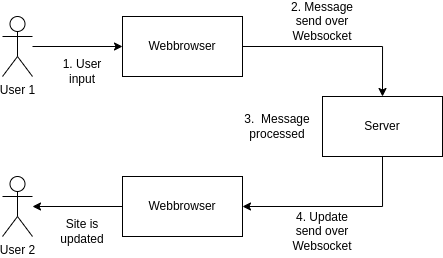
\includegraphics[width=0.6\linewidth]{websocketMessage.png}
    \label{fig:websocketMessage}
    \caption{Overview of the message handling.}
  \end{center}
\end{figure}
This means that user always view up to date data, while in old system users might operate on out of date data, if another user have altered that data.
The new system should be hosted hosted on \GLS{CIMT} servers, which would be in line with Rigshospitalet policies regarding software.

To ensure that the new tracershop handles message correctly behavior and follows requirements of \GLS{gmp}. The message is p in a three step plan seen below:
\begin{figure}[ht]
  \begin{center}
    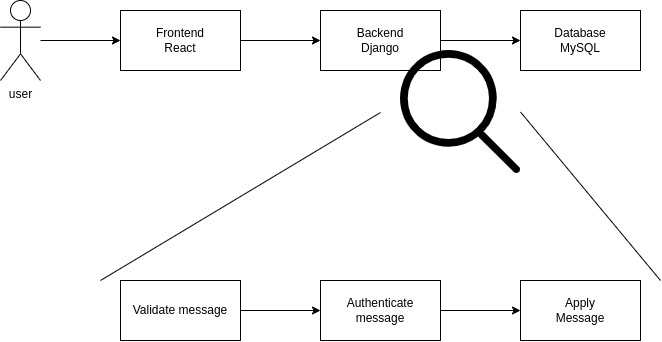
\includegraphics[width=0.6\linewidth]{MessageHandeling.png}
    \caption{Message handling by the backend}
    \label{fig:messageHandle}
  \end{center}
\end{figure}

\begin{enumerate}
  \item Validate the message - ensure that the message is correctly formatted and therefore would not cause an error if processed by the web server.
  \item Authenticate the message - Now the server can assume, the message is of a valid structure and determine it type.
  Then it can check if the authenticated user is allowed to complete such a message.
  \item Apply the message - Now the message is both valid and authorized, so the server will handle the message.
\end{enumerate}
Since the frontend doesn't have any contact with the database,
it is sufficient to ensure that the backend handles the users messages correctly.
This is done by a series of unit tests and end to end tests, which have a 95\% code coverage.
Which means that there's a program, which creates a test environment and run a number of tests where 95\% of all statement in the program is executed at least once.
Having above 90\% code coverage is considered good coverage as not all code is easily testable, nor does a code coverage of 100\% ensure that the program have no errors.
The testing proves the web server with high confidence handles messages correctly.\\
The django application has its own database to keep track of user session, which have been extended to to include general web site configuration.
This means that the django application database doesn't contain any records of orders or customers. This allows easy creation of test environments,
since the record database is a field in the django database, it can be easily exchanged to a connection to a database with a test environment.
The websocket requires a Regis database to broadcast messages.

\section*{New login system}

The new tracershop system uses an external authentication system, provided by the Capital region called BAM ID, managed by \GLS{CIMT}. All members of staff working in the capital region
have a BAM ID login. This login have various security features build in, such as automatic deprecation of passwords and minimum complexity requirements to passwords.
Secondary tracershop doesn't need store passwords and can rely on \GLS{CIMT}s services for password reset and deactivation of inactive accounts.\\
All users in the new tracershop are personal and have a role. These are divided into 3 catagories.

\begin{itemize}
  \item Shop - Users ordering tracers
  \item Production - Users producing tracers
  \item Admin - Users administrating the site, otherwise detached from both ordering and production of tracers
\end{itemize}

In addition there's different user subgroups that enable different features within tracershop.\\
The groups are as follows:

\begin{itemize}
  \item Shop - External - The user isn't an employee of the Capital region and doesn't have BAM ID. They can view their assigned customer's orders and order tracer authorized to the customer.
  Each of these user are connected to an external customer. The user is managed by an production admin.
  \item Shop - Internal - This is an employee of the Capital region and therefore have a BAM ID. A user is associated with one or more internal customers. This user is managed by a "Shop Superuser" user.
  \item Shop - Superuser - This is an internal shop user with additional rights to modify the automatic generated order based on a RIS booking.
  They can grant an internal user access to the same customers that they moderate.
  \item Production - User - The user can view orders from all customers and release tracer of authorized types.
  \item Production - Admin - Everything the production user can. Grant release rights to other production users, create new tracers, allow tracers to ordered by customers, and
  manage external user.
  \item Site Admin - The equivalent of a root user. The user can mimic all the functionality of other roles. The user isn't intended to use tracershop only to support it.
\end{itemize}

A shop user is associated and represent a number of customers. These associations are managed by the various admins and superusers of the site.

\section*{Test highlight}

To ensure correctness of tracershop, 

In general the validation of Tracershop doesn't concern themselves with \gls{incorrect data} since, the defining feature of incorrect data is,
that it doesn't break any restrictions placed upon the the system, but doesn't reflect reality. The implication is that tracershop cannot detect incorrect data.
The only method to combat \gls{incorrect data} is to allow users to modify data.\\
Tracershop is a bookkeeping tool not a measuring tool. It's the various measuring tools responsibility to measure correctly, which should have their own risk assessment and quality assurance.

\begin{itemize}
  \item \texttt{websocket.tests.test\_Consumer\_end\_2\_end.test\_GreatState}\\
  Ensures that when a user connects they receive a correct image of the database.
  \item \texttt{websocket.tests.test\_Consumer\_end\_2\_end.test\_free\_vial\_dependant\_orders}\\
  Ensures that an activity order is freed correctly.
  \item \texttt{lib.tests.tests\_pdfGeneration.test\_PDF\_Order}\\
  Ensures that the generated pdf matching the Activity Order. This test require manual verification since pdf files are not an easily parsed format.
  \item \texttt{lib.tests.tests\_pdfGeneration.test\_PDFInjectionOrder}\\
  Ensures that the generated pdf matching the Injection Order. This test require manual verification since pdf files are not an easily parsed format.
  \item \texttt{frontend.src.tests.components.ProductionPages.ActivityTable.White Box Order Rendering}\\
  Ensures that order data is displayed correctly.
\end{itemize}

\section*{Risk assessment}
A risk assessment is a collections of risks. Each risk consists of:
\begin{itemize}
  \item A description of the risk.
  \item A likelihood of how likely an incident is to occur.
  \item A damage estimate of an incident.
  \item A plan of action if an incident happen.
\end{itemize}
This risk assessment doesn't include production related risks such a dropped vial, or tracers not passing quality assurance.
The dispenser and the program transferring data have not modified by the new Tracershop, and therefore derives its validity from previous risk assessments.
See document number.: CVP-PROD-TS-001-14.01 in D4, for the latest validation of the dispenser.

\begin{itemize}
  \item Loss of a server.
  \begin{itemize}
    \item[Description] - A hosting server might become unavailable for a number a reasons:
      A foreign threat might encrypt the entire server, hardware failure, or a critical files might become corrupted due to aging hard drive.
      This is not an exhaustive list of reasons for server loss however other factors have minimal likelihood.
      It's beneficial to have plan of action in the event of an incident caused by an unknown risk.
    \item[Likelihood] - Low to medium - Currently the service runs on old hardware, insecure protocols and outdated software,
    which raises the likelihood of an incident occurring.
    Switching to \GLS{CIMT} hosted service with the new web server will eliminate these problems and thus reduce the risk.
    \item[Damages] - Medium to critical - Currently if a server becomes unavailable the source code to the original tracershop is lost.
    This means that restoration of the old system is impossible and any records made since the last backup would be lost.
    Due to the daily backup, an estimate of lost order would be up to 20.\\
    In the event, that both the backup PC and the server would become unavailable simultaneously all records would be lost.
    Due to the fragility of the dispenser script, automated import of vial data could become unavailable.
    \item[Plan] - In the event of server loss, if the loss was coursed by faulty hardware, repairing the server hardware might be possible and could restore the system to a pre-incident state, within 1-5 working days.
    If that's not possible to repair a new server is required. Assuming that the system is not deployed on \GLS{CIMT}s services and a spare server is not available,
    procuring a new server would take between 4-12 weeks with a 1 week installation period afterwards.
    If the server is virtualized and backed up, and the back ups are not lost, then the downtime would be around 1 day, which \GLS{CIMT} does.\\
    If the original source code is lost, the new web server would be forced to be used.
    Note that the new solution doesn't suffer the same vulnerability due to be hosted on github.
    In the case where github becomes unavailable, a replacement service would not be difficult to find as github is build around \Gls{git}.
  \end{itemize}
  \item Database is brought into an invalid state or incorrect state.
  \begin{itemize}
    \item[Description] - Due to the fact that it's the application responsibility to ensure correctness of the database, this is a risk.
    If the record database is in an invalid state, undefined behavior might occur because some data is invalid.\\
    Consider an example where a tracer is deleted. All orders with that tracer can no longer be determined to be of that tracer.
    \item[Likelihood] - Low - The web services doesn't allow, the user to perform arbitrary SQL queries,
    only predefined queries that take the database from one valid state to another valid state.
    It's difficult to ensure all possible user inputs, so it's possible that a user query might bring the database into an invalid state.
    An incident could occur if a system administrator creates a query that brings the database is into an invalid state.
    \item[Damages] - None to Low - The new tracershop can handle invalid database entries to an extend,
    meaning tracershop still works for unrelated entires and therefore not take the service down.
    The system will instead display, that certain information is undefined or not display the incorrect data at all.
    If the invalid state persist unnoticed for more 1 day the backup will be over written and the damage made permanent.
    However in such a case, it's unlikely to critical data, that have been corrupted.
    \item[Plan of action] - Upon notice a system administrator would enter the database and create a query to revert the database into a valid state.
    All queries made by tracershop to the record database is logged,
    which can greatly help system administrator to undo the damage.
    If the system administrator unable to restore the data using a query, then the plan switches to rollback to a backup of the record database, causing 1 days worth of data loss.
  \end{itemize}
  \item Incorrect user input
  \begin{itemize}
    \item[Description] - Tracershop have a number of fields, where the user must write some data in. Because it's humans that write this data, the system is subject to human error.
    It's incredible difficult to prevent this as there's nothing inherently wrong with \gls{incorrect data} user input. This also includes whenever a user forgets to update a piece of data.
    \item[Likelihood] - Very high. Humans use this program, no further elaboration required.
    \item[Damages] - None to Low - Very often human error will be spotted even ever a fresh set of eyes is looking at the \gls{incorrect data}.
    Whenever this happen the plan of action can be applied and most likely reverse any damage done. Incorrect data is also likely to cause other data become incorrect, however it's possible.
    \item[Plan] - The new tracershop allows user to edit non committed information their, and require users to sign in whenever they commit something to tracershop, while the information about to be committed is being displayed.
    Should the incorrect data be committed to the database, the personnel who finds the incorrect data should contact the system administrators and await their instructions.
    For instance if an order is committed with insufficient vials, the system administrator will request the personnel to create an additional order with the remaining vials.
  \end{itemize}
  \item The dispenser script stops working
  \begin{itemize}
    \item[Description] - As stated above, the program that ties the dispenser and database is highly fragile and could break, if the database is updated or if the hardcoded ip addresses changes.
    \item[Likelihood] - Low to medium - A user might accidental update the dispenser, or original server might be moved. However despite all of the alarm bells of fragility ringing, the system have been operating for 12 years.
    \item[Damages] - Low - The service would be very difficult to repair, due to the author of the program no longer working at Rigshospitalet, and is a forking perl script.
    However the loss of the service would not incorrect or \gls{invalid data} by itself. Only an additional source of error and additional human labor is required.
    \item[Plan] - Users would be forced to manually input data, that normally would have been transferred automatically and correctly.
  \end{itemize}
  \item Email server is unavailable
  \begin{itemize}
    \item[Description] - The email service is external, thus may for any reason be unavailable for an undefined amount of time.
    \item[Likelihood] - Unknown - The author have so limited experience with the available of the mail server, that a valid likelihood estimate is difficult to make.
    \item[Damages] - None to low - Customers are required to wait for confirmation that the tracer passed quality assurance mandated by \GLS{gmp}, so if the email server is down, the customer can not be notified through email.
    \item[Plan] - Due to websockets, updates to orders can be seen on tracershop in real time. Additionally users can download the email from tracershop from the associated order if needed or internal bookkeeping without any emails involved.
  \end{itemize}
  \item Malicious usage of tracershop
  \begin{itemize}
    \item[Description] - A user of tracershop attempt to sabotage the site.
    \item[Likelyhood] - Minimal - Users both staff and customers are verified users, which minimizes the risk of malicious usage.
    \item[Damages] - Low - Even in the event of that a user some how manages to destroy the record database, the backup is stored externally and thus not subject to any attack by the malicious user.
    \item[Plan] - All account are Personal.
    Critical actions such as freeing orders are audit logged. Allowing system administrator to identify the malicious user.
    There's a detection of SQL injections before the execution of each query.
  \end{itemize}
\end{itemize}


\section*{Conclusion}
The old tracershop fulfils the requirement set forwards by \GLS{gmp} annex 11, but is running on modules that have reached end of life.

A new system is proposed, that fulfils \GLS{gmp}, no longer uses, and improves various aspects of the tracershop system.
An extensive test sweep ensure that the django web server handles messages correctly.






\clearpage

\printglossary[type=main,style=long,nonumberlist]
\end{document}